\chapter{Evaluation}   \label{ch:6:eval}

In this section, the main body of work is evaluated based on objectives defined at the beginning of the project (Section \ref{objectives}) and are detailed as follows:
\begin{enumerate}
    \item Investigate the effect of different pre-processing techniques on semantic clustering and topic modelling.
    \item Investigate the effect of different word embedding models on the quality of clustering.
    \item Investigate the effect of different word embedding models and runtime environments on the performance (in terms of time efficiency).
    \item Evaluate the legibility of the results from the Topic Extraction Engine and Semantic Triple Extraction Engine based on user feedback.
\end{enumerate}

\section{Quantitative evaluation of semantic clustering} \label{s:evaluation_semantic_clustering}

\subsection{Effect of different processing techniques on clustering} \label{s:preprocess_clustering}

In order to cluster the news articles, different pre-processing techniques were applied to the article corpora in the Topic Extraction Engine (See~\Cref{s:procesing_topic_engine}) as a prerequisite for article vector generation for semantic clustering. These techniques included coreference resolution (CR), lemmatisation, stopword removal and named entity removal. The motivation behind this was to gauge the effect of these techniques on the silhouettes scores and incorporate those that the result in the most optimal scores, thereby resulting in improved clustering. \Cref{fig:pre-processing_sil} illustrates how omitting these different pre-processing techniques affects the silhouette score of the semantic clustering obtained for the Year-Category data group: Travel 2021. We can see that not doing any pre-processing (`No pre-processing') on the articles in Travel 2021 results in a poor silhouette score of 0.36 compared to `All', which results in a silhouette score of 0.691 and involves performing coreference resolution, lemmatisation, named entity and stopword removal. A silhouette score near 1 indicates dense, nicely separated clusters, while a score near 0 indicate significant cluster overlap (i.e., distance between them is insignificant). \Cref{fig:pre-processing_sil} shows the general trend that omitting any of these pre-processing techniques deteriorates the quality of clustering, by resulting in poor silhouette scores which indicate overlapping clusters.

\begin{figure}[H]
\centering
  \begin{minipage}[t]{.49\linewidth}
    \centering
    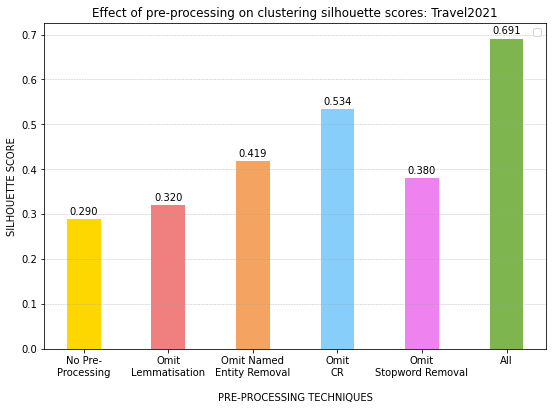
\includegraphics[width=\linewidth]{images/eval/effect_preprocessing.png}
    \caption{-}
    \label{fig:pre-processing_sil}
  \end{minipage}
  \begin{minipage}[t]{.49\textwidth}
    \centering
    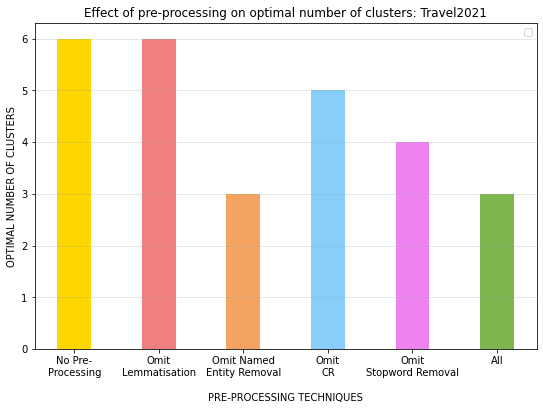
\includegraphics[width=\linewidth]{images/eval/preprocessing_cluster_no.png}
    \caption{-}
     \label{fig:pre-processing_cluster_no}
  \end{minipage}
\end{figure}

Another interesting observation as seen in~\Cref{fig:pre-processing_cluster_no} is how pre-processing affects the optimal number of clusters determined by the Topic Extraction Engine by running the KMeans clustering algorithm with a range of different `k' (See~\Cref{s:optimal_clusters}) and the optimal `k' (number of clusters) as the one that gives the highest silhouette score. Generally, the aim is to get the best silhouette score with the smallest number of clusters. This is because we do not want the Topic Extraction Engine to over-cluster the data by fixating on small differences within the corpus. The semantic clusters are derived for topics to be modelled within them, therefore, we want the engine to achieve a high-level semantic grouping of articles in the form of few, substantially large, distinct clusters. In the example shown in~\Crefrange{fig:pre-processing_sil}{fig:pre-processing_cluster_no}, Travel 2021 was selected as it has a very few number of member articles: 17. Not performing any pre-processing results in 6 clusters for a group of 17 articles. This is excessive as it means each semantic cluster has about 2 or 3 articles. Therefore, the latent topics extracted from these will be modelled on an extremely small corpus of about 2 articles and will most likely be incoherent. For the same data group, performing all the techniques mentioned (i.e., coreference resolution, lemmatisation, named entity and stopword removal), results in a much lower number of clusters: 3. In conclusion, the trend established by \Crefrange{fig:pre-processing_sil}{fig:pre-processing_cluster_no} \hl{is that by performing the pre-processing techniques mentioned , the engine is able to cluster the articles in a Year-Category group in fewer as well as more distinct clusters indicated by the lower optimal number of clusters and higher silhouette scores.}

% \todonum[inline]{Add LDA}

\subsection{Effect of filtering by POS tags on clustering} \label{s:pos_clustering}
% \todonum[inline]{And LDA}
Another key decision made in the Topic Extraction Engine in an attempt to improve the clustering of the input data was to filter the tokens extracted from the articles by their Part-Of-Speech (POS) tags. The decision was made to only use nouns tokens to represent each article. As mentioned earlier, in order to obtain the optimal number of clusters (optimal `k'), the engine performs Kmeans clustering with different values of `k', choosing the one which results in the highest silhouette score. \Crefrange{fig:pos_business2020}{fig:pos_pursuit2021} show the optimal cluster number and silhouette score for the Year-Category data groups: Business2020, Business2020, Politics2021 and Pursuit2021 when allowed POS tags are just `NOUN' and when they are `NOUN', `VERB', `ADJ' and `ADV'. These figures highlight the general trend that having a noun only tokens list to represent the articles for generating article vectors (for semantic clustering) gives a higher silhouette score with a smaller number of clusters. For instance, in~\Cref{fig:pos_business2021}, the silhouette score for noun only tokens list is 0.59 compared to 0.48 when tokens list contains nouns, adjectives, verbs and adverbs, resulting in a 23\% improvement in silhouette score and indicating better clustering for noun-only tokens list. The same is true for \Crefrange{fig:pos_politics2021}{fig:pos_pursuit2021} which show an 8.3\% and 16.3\% improvement respectively for clustering articles based on noun-only article corpus.

\begin{figure}[H]
\centering
  \begin{minipage}[t]{.49\linewidth}
    \centering
    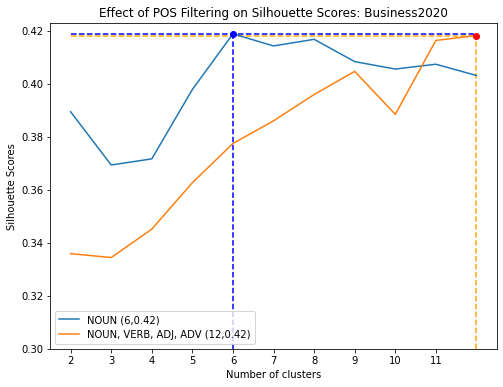
\includegraphics[width=\linewidth]{images/eval/business2020_sil.png}
    \caption{-}
    \label{fig:pos_business2020}
  \end{minipage}
  \begin{minipage}[t]{.49\textwidth}
    \centering
    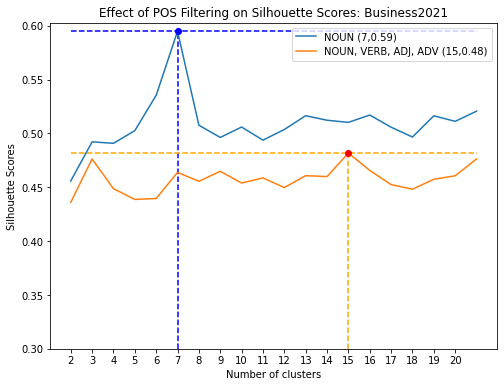
\includegraphics[width=\linewidth]{images/eval/business2021_sil.png}
    \caption{-}
    \label{fig:pos_business2021}
  \end{minipage}
  \begin{minipage}[t]{.49\textwidth}
    \centering
    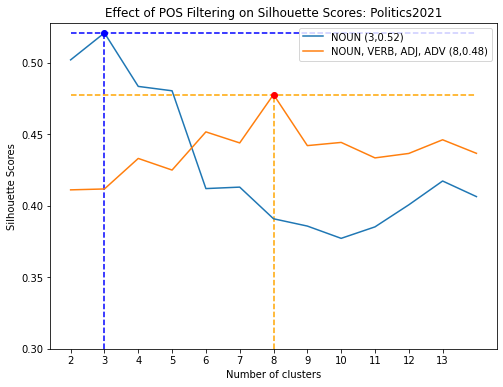
\includegraphics[width=\linewidth]{images/eval/politics2021_sil.png}
    \caption{-}
    \label{fig:pos_politics2021}
  \end{minipage}
  \begin{minipage}[t]{.49\textwidth}
    \centering
    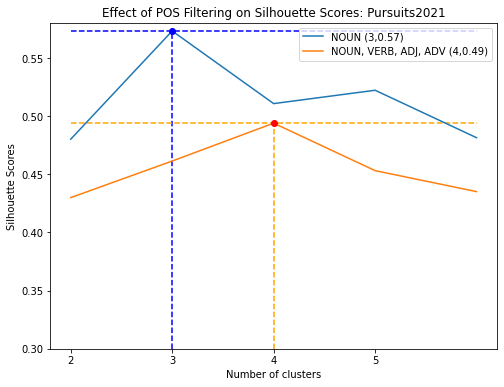
\includegraphics[width=\linewidth]{images/eval/pursuits2021_sil.png}
    \caption{-}
    \label{fig:pos_pursuit2021}
  \end{minipage}
\end{figure}

More evidently, it is important to note that the optimal number of clusters is much lower with a noun-only corpus as seen in the figures above. \Cref{fig:pos_business2020} shows that the silhouette score of 0.42 is achieved with only 6 clusters for noun-only tokens list compared to 12 clusters with nouns, adjectives, verbs and adverbs. For example, \textit{['coronavirus', 'aviation', 'industry', 'border', 'restriction', 'travel, 'quarantine']} is a more concise and general representation of an article as opposed to \textit{['job', 'wipe', 'bad', 'come', 'worker', 'tell', 'worker', 'coronavirus', 'spend', 'lengthy','drastically', 'quarantine']}. Adjectives, adverbs and verbs are not meaningful on their own. Additionally, their generic nature means they are not unique to articles and including them in the \texttt{filtered\_tokens} allows them to equally contribute to their corresponding article vectors as distinctive nouns (e.g., `pandemic') in the corpus, thereby making the article vector less precise. Furthermore, the more tokens used for generating the document vectors, the greater the potential to introduce noise, resulting in high variance among vectors, making the corpus difficult to cluster, and thereby resulting in suboptimal clustering (with more clusters than necessary).

\subsection{Effect of different word embedding techniques on clustering} \label{s:word_embeddings}

\begin{figure}[H]
\centering
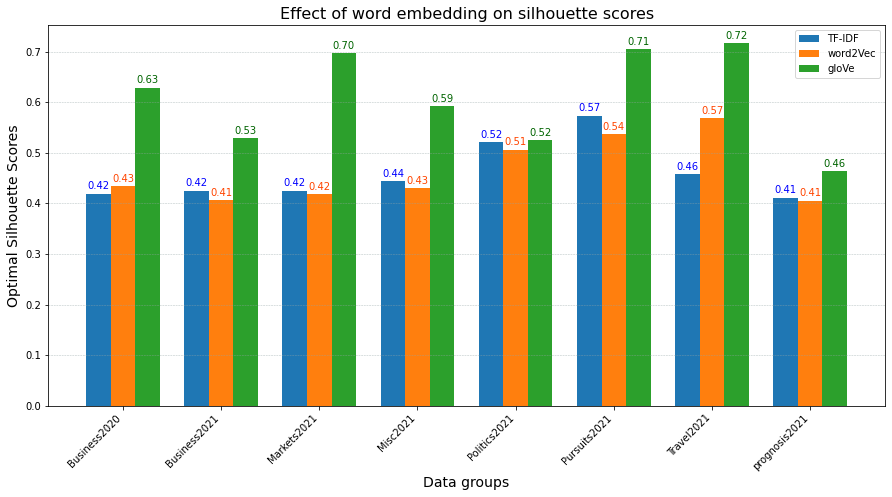
\includegraphics[width=0.7\linewidth]{images/eval/word_embedding.png}
\caption{Effect of using TF-IDF, Word2Vec and GloVe as word embedding model on clustering silhouette scores}
\label{fig:word_embed}
\end{figure}
\vspace{-1em}
As discussed in~\Cref{word_embed_approaches}, in order to cluster the articles, each article's corresponding list of \texttt{filtered\_tokens} is vectorised. \Cref{fig:word_embed}, highlights the effect of the different word embedding techniques, in particular, TF-IDF, Word2Vec and GloVe on the silhouette scores of clusters thereby providing a quantitive measure of how the `goodness' of semantic clustering is influenced by the word embedding approaches. As indicated by the bar chart in Figure \ref{fig:word_embed}, using GloVe to vectorise the articles gives a major improvement in the silhouette scores across all the Year-Category input groups, compared both to TF-IDF and word2Vec.

\begin{table}
\centering
\renewcommand{\arraystretch}{1.05}
\begin{tabularx}{0.7\textwidth}{X X X} 
\multicolumn{3}{c}{GloVe Percentage Improvement} \\
 \hline
 Data group & TF-IDF & Word2Vec \\
 \hline
 Business 2020 & 50.14\% & 45.02\%  \\ 
 Business 2021 & 24.45\% & 30.13\%  \\
 Markets 2021 & 63.91\% & 66.68\% \\
 Misc 2021 & 33.40\% & 37.81\% \\
 Politics 2021 & 0.76\% & 3.71\% \\
 Pursuits 2021 & 23.06\% & 31.41\%  \\ 
 Travel 2021 & 56.58\% & 26.11\% \\
 Prognosis 2021 & 12.72\% & 14.32\% \\ 
 \hline
 Average & 33.13\% & 31.90\% \\ 
\end{tabularx}
\caption{Percentage improvement for silhouette scores when using GloVe over TF-IDF and Word2Vec for all Year-Category data groups}
\label{table:word_embed}
\end{table}

Table \ref{table:word_embed} shows the (percentage) improvement in silhouette scores when using GloVe over TF-TDF and Word2Vec. We see a 33.13\% improvement in clustering (by means of improved silhouette scores) when using GloVe instead of TF-IDF and 31.90\% improvement when compared to word2Vec. Based on these results, it is evident that using GloVe is the optimal approach for word embedding for token vectorisation for semantic clustering. Additionally, we gain confidence in using GloVe as the silhouette scores for the clustering of most input groups are around 0.7 (as seen in~\Cref{fig:word_embed}) which shows evidence of distinct clusters of articles. When clustering news articles, especially articles pertaining to a specific industry within a category, obtaining a perfect clustering with silhouette score of 1 is not realistic, as there is bound to be common underlying themes resulting in some overlap.
% \todonum[inline]{FOR TOPIC MODELLING Do a comparison TABLE for the different sets of allowed postags, Remove adjective noun gives better performance, can show in sil score}

\section{Quantitative evaluation of topic modelling} \label{s:evaluation_topic_extraction}

\subsection{Effect of pre-processing on topic modelling} \label{s:preprocess_topic}

\begin{figure}[H]
  \centering
    \begin{minipage}[t]{.49\linewidth}
      \centering
      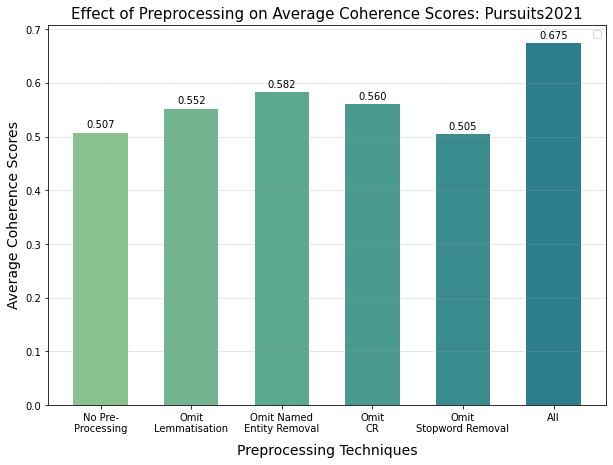
\includegraphics[width=\linewidth]{images/eval/coherence_preprocess.png}
      \caption{-}
      \label{fig:preprocess_topic}
    \end{minipage}
    \begin{minipage}[t]{.49\textwidth}
      \centering
      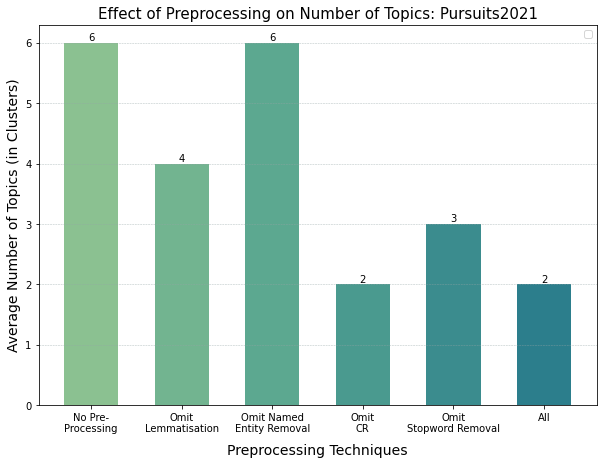
\includegraphics[width=\linewidth]{images/eval/preprocessingTopicNo.png}
      \caption{-}
       \label{fig:pre-processing_topic_no}
    \end{minipage}
  \end{figure}

 Similar to~\Cref{s:preprocess_clustering}, this section also focuses on the effect of pre-processing techniques but on the topics extracted from semantic clusters in Year-Category groups. The topics extracted from each cluster result in a topic coherence score and these are averaged over all clusters in a Year-Category input group to give an average coherence score (for the input group). The coherence score is a useful metric for evaluating the quality of topics extracted as it assesses the degree of semantic similarity between high-scoring terms in a single topic. In similar trends as seen for semantic clustering,~\Crefrange{fig:preprocess_topic}{fig:pre-processing_topic_no} show that applied all the pre-processing techniques (represented by the 'All' bar) results in a significantly higher average coherence score with less number of topics compared to other approaches.  

In the case of omitting coreference resolution, the (average) coherence score falls (to 0.560) as word tokens such as 'it', 'they', 'those' (essentially, unresolved pronouns) do not contribute to the semantic similarity with other high scoring terms in the corpus. Therefore, resolving these pronouns to their respective nouns, means that the frequency of the nouns increases, and they are more likely to contribute to the topics in the corpus. Omitting lemmatisation similarly results in a drop in coherence (and increase in number of topics) as the tokens are not resolved to their base forms affecting the frequency of common words (e.g. tourist and tourists will be treated as different keywords).

As mentioned in~\Cref{data_cleaning}, stopword list contains the default spaCy stopwords (around 326 words), augmented with a custom list of frequently occurring unnecessary words and phrases specific to the input data such as `told', `said' (as news article commonly quote entities, especially people) and `airline', `flight etc. (since news article are specific to the airline industry). The latter are removed as they can be thought of as overarching themes spanning many topics but do not contribute to a distinct topic. The idea is that we do not want the model to fixate on these commonly appearing contextless stopwords and output junk topics, hence why removing them results in better topic coherence (0.775 denoted by the \qs{All} bar) as seen in \ref{fig:preprocess_topic} compared to when they are retained which results in a lower topic coherence of 0.639.

As established prior, named entity removal is done to allow the engine to find distinct topics within a cluster that are not dependent on the named entities. For instance, let's assume that there is a huge overlap between \qs{pilot unions} and \qs{British Airways}. Retaining named entities in the input corpus could result in the model selecting `British Airways' as a topic instead of 'pilot unions'. \Cref{fig:pre-processing_topic_no}, indicates that retaining named entities significantly increases number of topics (6). Some of these topics are `junk', have low coherences scores implied by the lower average coherence score of 0.582 in~\Cref{fig:preprocess_topic}. This makes sense as named entities can be associated with several topics resulting in overlapping clusters, which may be split resulting in more (incoherent) topics. Finally, as expected, omitting all pre-processing results in the lowest average coherence score of 0.401 and highest number of topics (6). 

\subsection{Effect of filtering by POS tags on topic modelling} \label{s:pos_topic}

\begin{figure}
  \centering
    \begin{minipage}[t]{.49\linewidth}
      \centering
      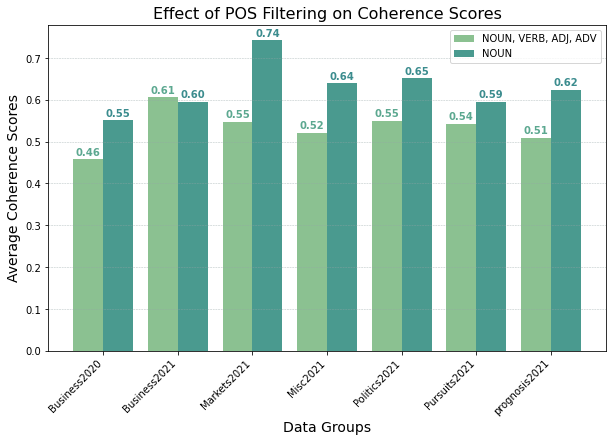
\includegraphics[width=\linewidth]{images/eval/pos_coherence.png}
      \caption{pos}
      \label{fig:pos_topic}
    \end{minipage}
    \begin{minipage}[t]{.49\linewidth}
      \centering
      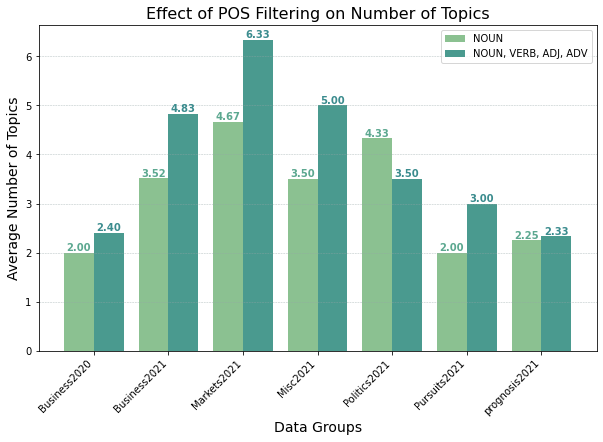
\includegraphics[width=\linewidth]{images/eval/topics_pos.png}
      \caption{-}
       \label{fig:topics_pos}
    \end{minipage}
  \end{figure}

The \texttt{filtered\_tokens} list (for each article) that was used to generate the article vectors for clustering, is passed to the LDA model to extract topics from each of the semantic clusters for a Year-Category group. In order to determine the effect of different allowed POS tags on the quality of topics extracted, the coherence score measure is used. From~\Cref{fig:pos_topic}, it is apparent that the noun only tokens approach to extract tokens performs better than when noun, adjectives, verbs and adverbs are used as the average coherence scores are generally higher for the former approach. Across all the data groups, we see an average coherence score improvement of 18.2\% with the noun only topic extraction approach. This is because, as mentioned in~\Cref{s:pos_clustering}, there are several generic adverbs, adjectives and verbs that occur across articles in high frequency. Including these in the LDA corpus for topic extraction increases the potential for the model to select these as keywords (high-scoring terms) for a topic. This would result in a low semantic similarity among the keywords in a topic, resulting in poor coherence score. The lack of similarity in the filtered tokens articles in LDA corpus would result in the model fitting to the noise, resulting in a higher number of incoherent `junk' topics. This is apparent from \Crefrange{fig:pos_topic}{fig:topics_pos} which show that using `NOUN, VERB, ADJ, ADV' results in lower coherence scores for higher number of topics.


\section{Time Efficiency}

\subsection{Comparing Runtimes in Various Environments}
\vspace{-1ex}

\begin{table}[H] 
\centering
\renewcommand{\arraystretch}{1.05}
\begin{tabularx}{\textwidth}{X X X X} 
 \hline
%  {\hsize=.25\hsize\linewidth=\hsize}Data group & {\hsize=.25\hsize\linewidth=\hsize}CPU & {\hsize=.3\hsize\linewidth=\hsize}Multiprocessing CPU & {\hsize=.2\hsize\linewidth=\hsize}GPU \\
Data group & CPU &  Multiprocessing (CPU) & Tesla T4 GPU \\
 \hline
 Business 2020  & 351.41  & 352.51  & 39.47 \\ 
 Business 2021  & 1713.60 & 1431.80 & 138.47 \\
 Markets 2021   & 839.75  & 1252.64 & 74.18\\
 Misc 2021      & 215.41  & 337.49  & 18.60 \\
 Politics 2021  & 856.42  & 1267.96 & 64.87 \\
 Pursuits 2021  & 178.54  & 377.49  & 15.00 \\ 
 Travel 2021    & 169.52  & 452.80  & 12.92 \\
 Prognosis 2021 & 583.33  & 888.27  & 51.63 \\ 
 \hline
 Total time (s) & 4907.98 & 1920.16 & 414.60 \\ 
 Total time (min) & 81.80  & 32.10 & 6.90\\ 
\end{tabularx}

\caption{Time taken to run the Semantic Analysis Engine pipeline for all data groups(in seconds)}
\label{table:cputime}
\end{table}
\vspace{-2em}
\Cref{table:cputime} shows the different runtimes for the pipeline when running on a CPU, with multiprocessing (on CPU) and GPU (Tesla T4). Ideally, the pipeline is meant to be run on the GPU as it results in significant improvement in computation time, with the whole process of running the pipeline for all the input groups from the dataloader taking only 6.9 minutes in comparison. This is 11.8 times faster than running it on the CPU and 4.6 times faster than running it on the CPU with multiprocessing. The reason for the high computation time for CPU is due to the expensive calls to the AllenNLP models, particularly the Fine-Grained NER, SpanBERT Coreference and RoBERTa Sentiment models (See~\Cref{s:models}), which unlike spaCy, are not built for production use and therefore not optimised for time. However, given that they are state-of-the-art models that achieve high performance for their respective NLP tasks, their use is extremely beneficial to the project. This motivated the use of multiprocessing and designing the engine architecture as a pipeline which takes an input Year-Category data group and outputs the results for the visualisation tool (See \Cref{fig:sys_arch}), to allow for feasible CPU computation. 

Processes are traditionally constrained to just having access to their own process memory, however shared memory permits data structures to be shared between processes. The AllenNLP models in question are significantly large and RAM-intensive and therefore, having multiple copies of the models (one for each process) can result in the machine running out memory. Therefore, it is crucial to store these models in shared memory in order to provide centralised access to all running processes and avoid redundant copies of models for each process. This allowed running the tool on the 8 different data groups simultaneously, resulting in a performance gain in terms of time efficiency as seen in~\Cref{table:cputime}, which shows that using multiprocessing results in 2.55 times lower computational time compared to running with single process CPU. This is because the idle time is significantly reduced by concurrent processes during the expensive calls for coreference resolution, sentiment analysis and NER. 

\subsection{Effect of different word embedding models on GPU runtime}
\vspace{-1ex}
\begin{table}[H]
\centering
\renewcommand{\arraystretch}{1.05}
\begin{tabularx}{0.9\textwidth}{X X X X} 
\multicolumn{4}{c}{GPU runtime (in seconds)} \\
 \hline
 Data group & TF-IDF & Word2Vec & GloVe \\
 \hline
 Business 2020 & 44.67& 33.82& 39.47 \\ 
 Business 2021 & 256.19 & 130.56 & 138.47 \\
 Markets 2021 & 87.30 & 75.00 & 74.18 \\
 Misc 2021 & 16.67 & 17.92 & 18.60 \\
 Politics 2021 & 60.72 & 71.06 & 64.87 \\
 Pursuits 2021 & 15.00 & 14.38 & 15.00 \\ 
 Travel 2021 & 13.06 & 12.85 & 12.92 \\
 Prognosis 2021 & 53.61 & 59.39 & 51.63 \\ 
 \hline
 Total time (s) & 414.98 & 547.92 & 414.60 \\ 
  Total time (min) & 6.92 & 9.12 & 6.90 \\ 
\end{tabularx}
\caption{Time taken to run the pipeline (on GPU) with different word embedding models}
\label{table:word_embed_time}
\end{table}

\vspace{-3ex}
\Cref{table:word_embed} highlights the effect of different word embedding models on the time taken to run the Semantic Analysis Engine pipeline on the Tesla T4 GPU for all data groups. As established in \Cref{s:word_embeddings}, the Topic Extraction Engine uses \texttt{GloVe} as the word embedding model as it gives a significant improvement in the semantic clustering silhouette scores. Furthermore, it also results in more efficient (faster) computation when running the pipeline for all input data with a total runtime of 414.60 seconds, which is 31.15\% lower than using \texttt{Word2Vec}. The difference in runtimes for when using \texttt{TF-IDF} and \texttt{GloVe} is trivial, however, given the 33.13\% improvement (See~\Cref{fig:word_embed}) in silhouette score of \texttt{GloVe} over \texttt{TF-IDF}, \texttt{GloVe} proves to be the best approach in terms of time efficiency and optimal clustering. 

\section{Qualitative User Evaluation} \label{s:user_eval}
In an attempt to gain a greater understanding of the performance of our tool, user testing was conducted with a focus group of 7 people, including members from DeepSearchLabs to obtain qualitative evaluation for visualised results from the Topic Extraction Engine and Semantic Triple Extraction Engine.

\begin{figure}[H]
\centering     %%% not \center
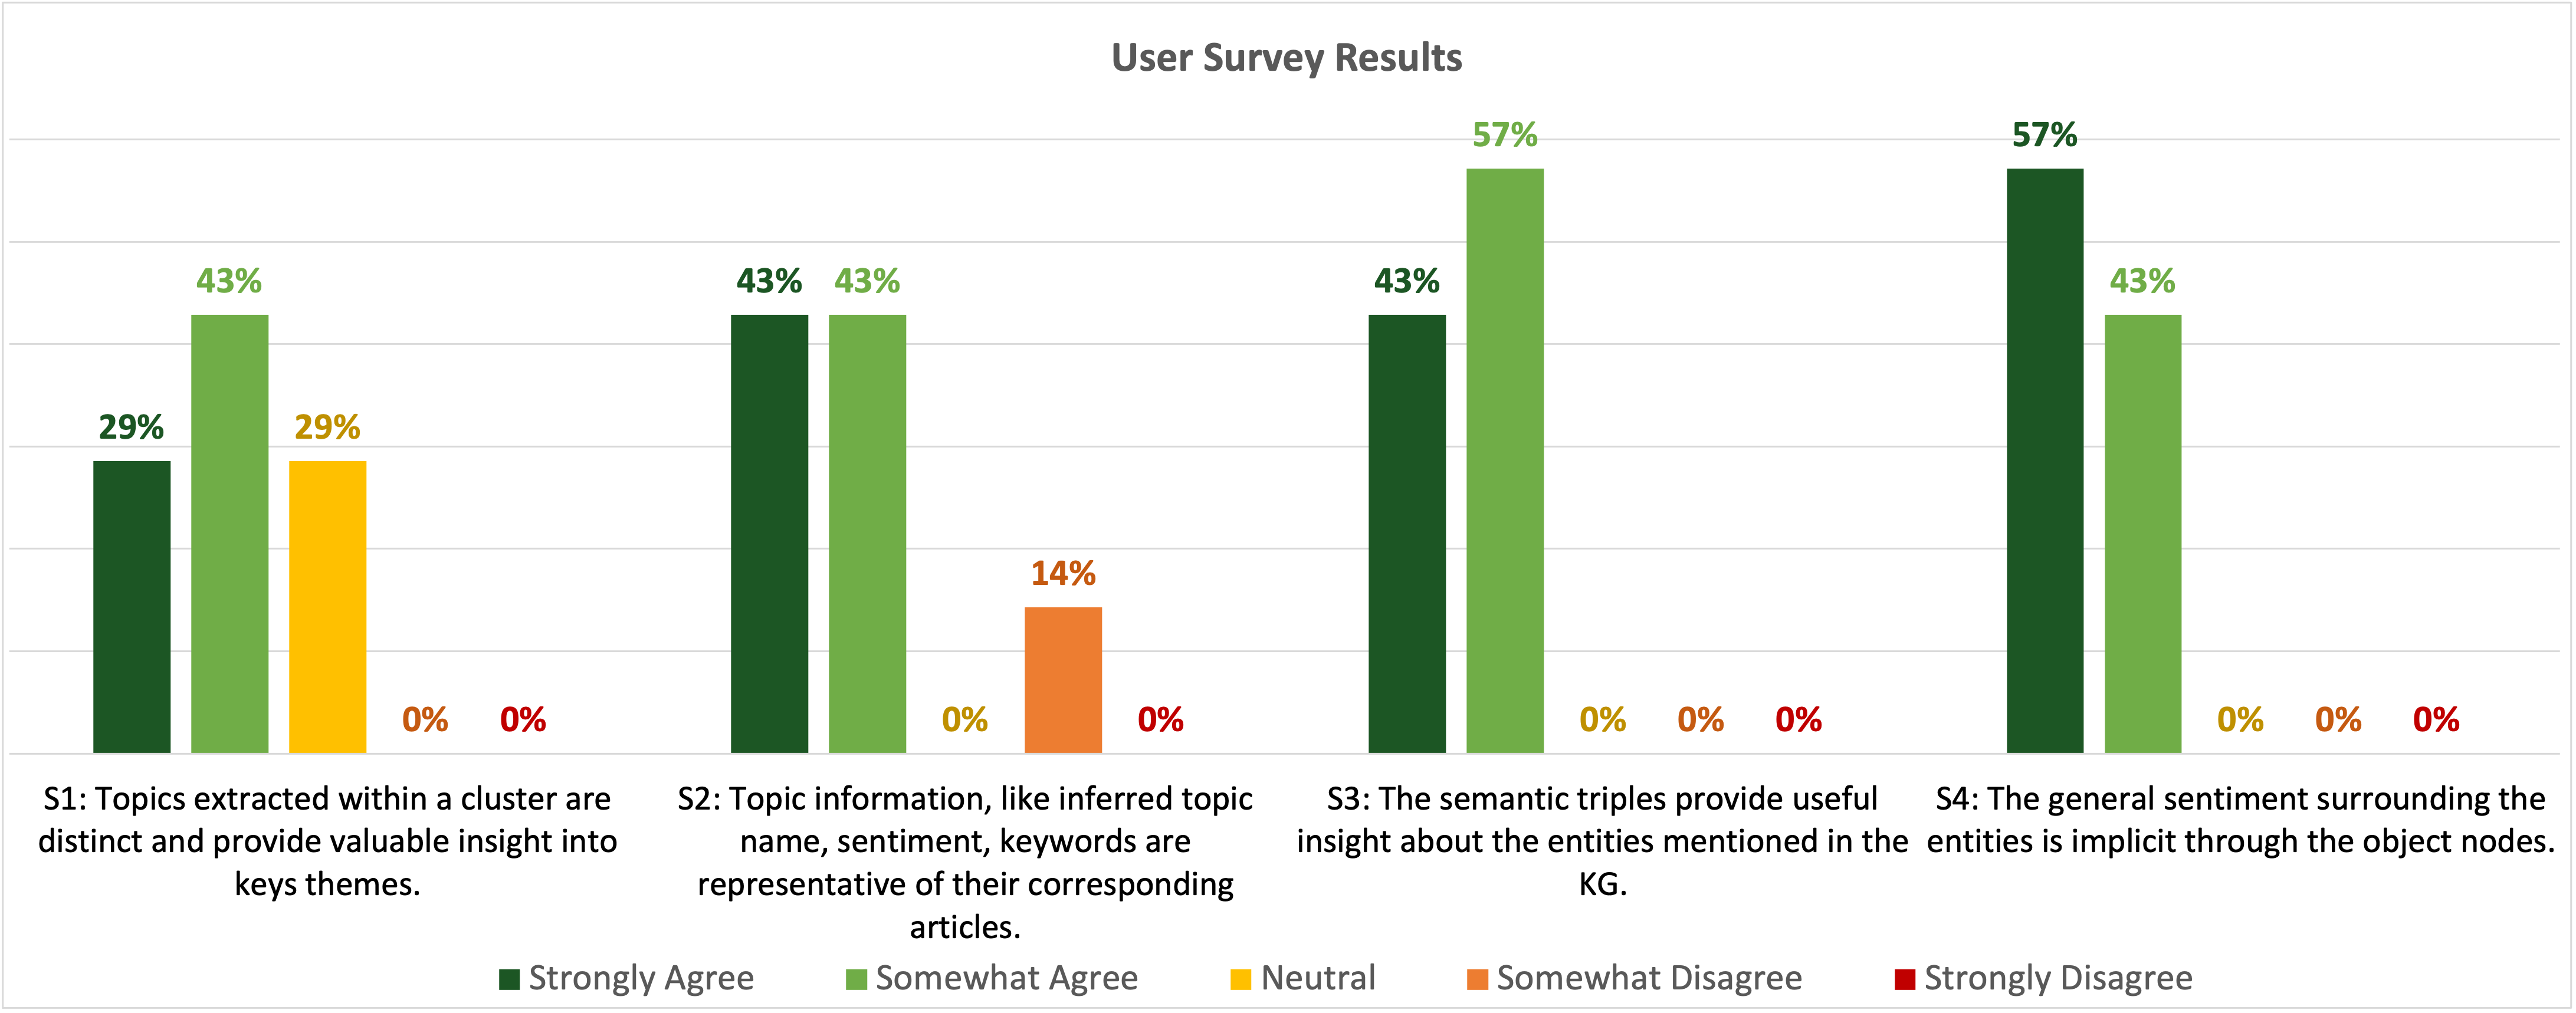
\includegraphics[width=0.95\linewidth]{images/eval/user_eval.png}
\caption{E-}
\label{user_eval}
\end{figure}

The evaluation was conducted in the form of a survey where the users were asked score their agreement for 4 statements based on 5 point scale. In order to ensure uniformity to get a more accurate user perception of the tool, the respondents were asked to focus on the results for the Year-Category input group Travel 2021. \Cref{user_eval} shows the response summary for the 4 statements, where S1 and S2 focus on the cluster-topic graphs for displaying results from Topic Extraction Engine and S3 and S4 focus on the force-directed (knowledge) graph for displaying triples from the Semantic Triple Extraction Engine. 

The responses show that over 72\% of the respondents agree (though only 29\% strongly agree) with statement 1 (S1) that the Topic Extraction Engine is able to extract fairly distinct, coherent latent topics from the semantic clusters, with the other 29\% remaining indifferent. For S2, while 86\% respondents agree that the articles within the topic make sense based on the topic information, 14\% (1 of 7) disagree. This is understandable, because as identified in~\Cref{limitation_topics}, assigning an article a single dominant topic may not always be intuitive. The responses for S3 and S4 were overwhelming positive, with a 100\% agreement for both statements verifying that the semantic triples in the graph provide useful insight about key entities (the relevance of entities depicted by the size of their nodes) and the general sentiment associated with these entities (depicted via green-red colour scheme for positive and negative sentiment respectively). Comparing the agreements responses for S1-S2 with S3-S4, we can infer the qualitative user evaluation gives greater confidence in the Semantic Triple Extraction Engine compared to Topic Extraction Engine, although both were received as there were no strong disagreements with any of the statements (which generalise some of the objectives of the engines). 
